% !TeX document-id = {2870843d-1baa-4f6a-bd0a-a5c796104a32}
% !BIB TS-program = biber
% !TeX encoding = UTF-8
% TU Delft beamer template

\documentclass[aspectratio=43]{beamer}
\usepackage[english]{babel}
\usepackage{csquotes}
\usepackage{calc}
\usepackage[absolute,overlay]{textpos}
\usepackage{graphicx}
\usepackage{subfig}
\usepackage{mathtools}
\usepackage{amsfonts}
\usepackage{amsthm}
\usepackage{comment}
\usepackage{siunitx}
\usepackage{MnSymbol,wasysym}
\usepackage{array}
\usepackage{qrcode}
\usepackage{hyperref}
\usepackage{physics}
\usepackage{qcircuit}

\setbeamertemplate{navigation symbols}{} % remove navigation symbols
\mode<presentation>{\usetheme[verticalbar=false]{tud}}

% BIB SETTINGS
\usepackage[
    backend=biber,
    giveninits=true,
    maxnames=30,
    maxcitenames=20,
    uniquename=init,
    url=false,
    style=authoryear,
]{biblatex}
\addbibresource{bibfile.bib}
\setlength\bibitemsep{0.3cm} % space between entries in the reference list
\renewcommand{\bibfont}{\normalfont\scriptsize}
\setbeamerfont{footnote}{size=\tiny}
\renewcommand{\cite}[1]{\footnote<.->[frame]{\fullcite{#1}}}
\setlength{\TPHorizModule}{\paperwidth}
\setlength{\TPVertModule}{\paperheight}

\newcommand{\absimage}[4][0.5,0.5]{%
	\begin{textblock}{#3}%width
		[#1]% alignment anchor within image (centered by default)
		(#2)% position on the page (origin is top left)
		\includegraphics[width=#3\paperwidth]{#4}%
\end{textblock}}

\newcommand{\mininomen}[2][1]{{\let\thefootnote\relax%
	\footnotetext{\begin{tabular}{*{#1}{@{\!}>{\centering\arraybackslash}p{1em}@{\;}p{\textwidth/#1-2em}}}%
	#2\end{tabular}}}}

% New commands (Giorgio)
\newcommand{\R}{\mathbb{R}}  % real set
% \newcommand{\pdv}[2]{\frac{\partial #1}{\partial #2}}
\newcommand{\inner}[2]{\langle #1,\, #2\rangle}
\newcommand{\kernel}[2]{\kappa\left( #1, #2 \right)}

\DeclarePairedDelimiter\ceil{\lceil}{\rceil}
\DeclarePairedDelimiter\floor{\lfloor}{\rfloor}


\title[]{Applied Quantum Algorithms - Lecture 9 - Quantum Kernel Methods}
\institute[]{Delft University of Technology, The Netherlands}
\author{Giorgio Tosti Balducci}
\date{May 3, 2023}


\begin{document}
\section{Introduction}
{
\setbeamertemplate{footline}{\usebeamertemplate*{minimal footline}}
\frame{\titlepage}
}

\begin{frame}{Contents} % some commands, e.g. \verb require [fragile]
\begin{enumerate}
  \item Learning with quantum kernels
  \begin{enumerate}
    \item Quantum supervised ML models are kernel methods\cite{Schuld_2021_kernels}
    \item Learning the right metric
    \item Support Vector Machine (SVM)
    \item Comparing quantum kernels and variational QC models
  \end{enumerate}
  \item Demos on PennyLane and Qiskit
\end{enumerate}
\end{frame}

\section{Lecture}

\begin{frame}
  \frametitle{The density matrix representation of quantum states}
    As opposed to the vector representation.
\end{frame}


\begin{frame}
  \frametitle{Data encoding as a feature map in the $\rho(x)$ space}

  

\end{frame}


\begin{frame}
  \frametitle{Quantum kernels}
  \framesubtitle{a.k.a. inner products of quantum feature vectors}

  

\end{frame}


\begin{frame}
  \frametitle{Quantum kernels}
  \framesubtitle{Kernels induced by the data encodings we know}



\end{frame}


\begin{frame}
  \frametitle{Quantum kernels}
  \framesubtitle{Question 1}

  \centering
  \textcolor{red}{What does the kernel expression for \emph{basis encoding} tell us about how we can learn with it?}
  
  \ \\
  \emph{Tip:} think about classification

\end{frame}


\begin{frame}
  \frametitle{Quantum kernels}
  \framesubtitle{Question 2}

  \centering
  \color{red} Is (repeated) amplitude encoding the same as the classical polynomial encoding?

\end{frame}


\begin{frame}
  \frametitle{Back to quantum models}

  In lecture 8, we defined the supervised QML model as
  \[f(\mathbf{x}, \theta) = \ev{\mathcal{M}}{\psi\left( \mathbf{x}, \theta \right)},\]

  where
  \[\ket{\psi\left( \mathbf{x}, \theta \right)} = W\left( \theta \right) U(\mathbf{x}) \ket{0}.\]

  In density matrix representation
  \[f(\mathbf{x}, \theta) = \tr\left[ \ketbra{\psi\left( \mathbf{x},\theta \right)}\mathcal{M} \right] = \tr\left[\rho\left( \mathbf{x},\theta \right)\mathcal{M}\right]\]

  The parameters $\theta$ can be included in $\mathcal{M}_\theta$ (objective: find the optimal measurement). For the time being, however let's forget about them
  \[f(\mathbf{x})=\tr\left[\rho\left( \mathbf{x} \right)\mathcal{M}\right]\]

  In this way, \emph{our models are measurements in feature space}.

\end{frame}


\begin{frame}
  \frametitle{What Hilbert spaces are associated to a QML model?}

  \begin{enumerate}
    \item Feature space: $\left\{ \phi:\mathcal{X}\rightarrow \mathbb{C}^{4n}| \phi:\mathbf{x}\rightarrow \rho\left( \mathbf{x} \right) \right\}$
    \item Space of quantum models: $\left\{ f:\mathcal{X}\rightarrow\R| f\left( \mathbf{x} \right)=\tr\left[ \rho\left( \mathbf{x} \right)\mathcal{M} \right] \right\}$
  \end{enumerate}

  \ \\
  What is the relation between the two?
  \begin{block}{Theorem 1}
    Quantum models of the form $\tr\left[\rho\left( \mathbf{x} \right)\mathcal{M}\right]$ are linear models in the feature vectors $\rho\left( \mathbf{x} \right)\in \mathcal{F}$.
    \note{proof on whiteboard}
  \end{block}

  \begin{block}{Theorem 2}
    Measurements in feature space are linear combination of feature vectors
    \[\mathcal{M} = \sum_i \gamma_i \rho\left( \mathbf{x}^{(i)} \right)\]
    \note{proof on whiteboard}
  \end{block}

\end{frame}


\begin{frame}
  \frametitle{A Hilbert space induced by the kernel}
  \framesubtitle{The Reproducing Kernel Hilbert Space (RKHS)}
  
  Let's forget about quantum models for a moment and let's focus on \emph{kernels}. We can define a \emph{Hilbert} space $F$ induced by $\kappa\left( \mathbf{x}, \cdot \right)$

  \begin{exampleblock}{Reproducing Kernel Hilbert Space (RKHS)}
    The Hilbert space $F$ that is the span of the functions $g(\cdot)=\kappa\left( \mathbf{x}, \cdot\right)$ and where the inner product between $g(\cdot)=\sum_i \alpha_i \kappa\left( \mathbf{x}^{(i)}, \cdot\right)$ and $h(\cdot)=\sum_i \beta_i \kappa\left( \mathbf{x}^{(i)}, \cdot\right)$ is

    \[\inner{g}{h}_F = \sum_{i,j} \alpha_i \beta_j \kappa\left( \mathbf{x}_i, \mathbf{x}_j \right)\]
  \end{exampleblock}

  \ \\
  A bit more intuitively:
  \begin{itemize}
    \item The RKHS is the space that associates each data point with a \emph{function}, which is its distance measure (inner product).
  \end{itemize}
  
\end{frame}


\begin{frame}
  \frametitle{RKHS}
  \framesubtitle{Intuition}

  Gaussian kernel: $\kernel{\mathbf{x}}{\mathbf{x}^\prime} = e^{-\frac{\gamma}{2}\abs{\mathbf{x}-\mathbf{x}^\prime}^2}$

  \ \\
  \centering
  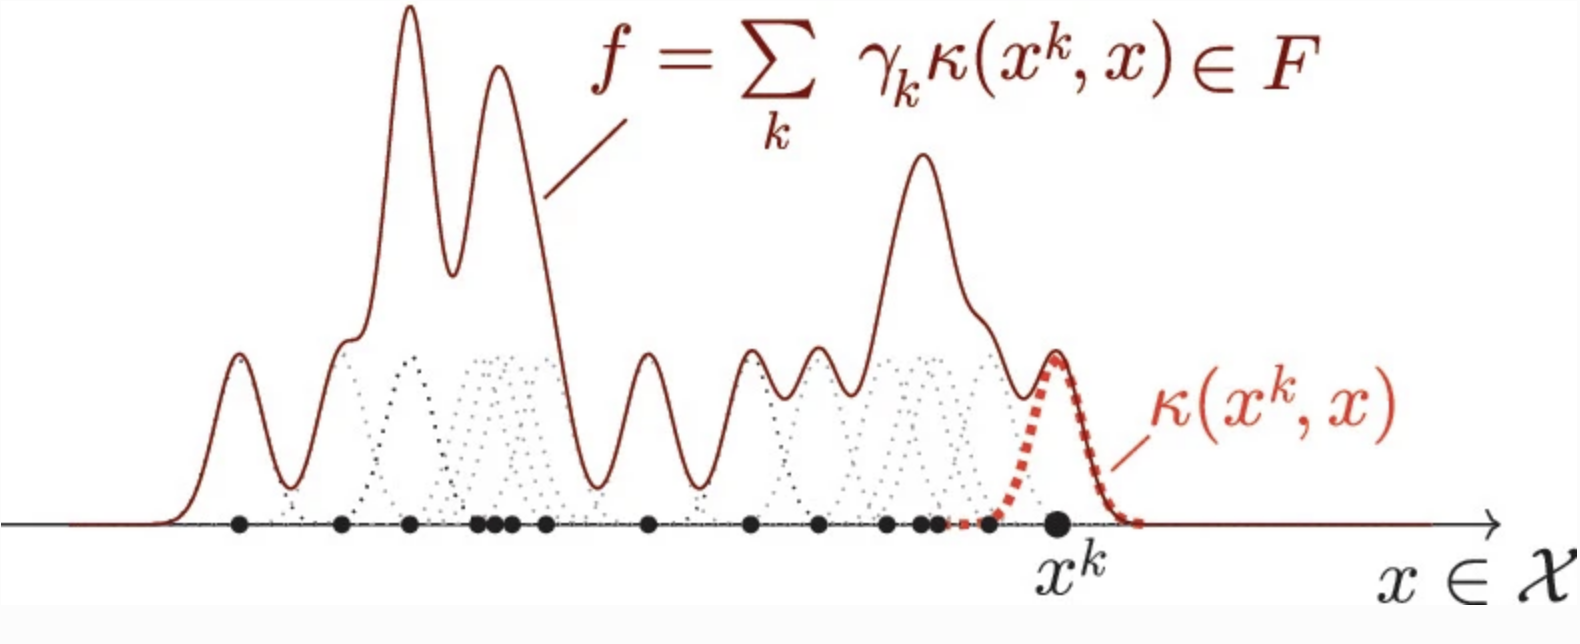
\includegraphics[width=.5\textwidth]{pics/schuld-rkhs-intuitive.png}

  By tuning $\gamma$, we tune how each point $\mathbf{x}\in \mathcal{X}$ `affects' (is similar to) each other.

\end{frame}


\begin{frame}
  \frametitle{RKHS}
  \framesubtitle{Why do we care?}

  But why bothering about the RKHS?\note{Becuase it contains all and the same functions as the space of models that are linear in the feature space! So the models defined as $\tr[\rho\left( x \right)\mathcal{M}]$}.

  \begin{block}{Theorem 3}
    Functions in the RKHS $F$ are linear models in the data-encoding features in $\mathcal{F}$ and vice-versa.
  \end{block}

  \ \\
  Therefore, if we can prove something about the RKHS induced by $\kappa\left( \mathbf{x}, \mathbf{x}^\prime\right)$, the same property holds for our quantum model $\tr[\rho\left( \mathbf{x} \right)\mathcal{M}]$.
  \begin{itemize}
    \item universality
    \item trainability
    \item generalization
  \end{itemize}

\end{frame}


\begin{frame}
  \frametitle{The vector spaces of quantum models}

  \centering
  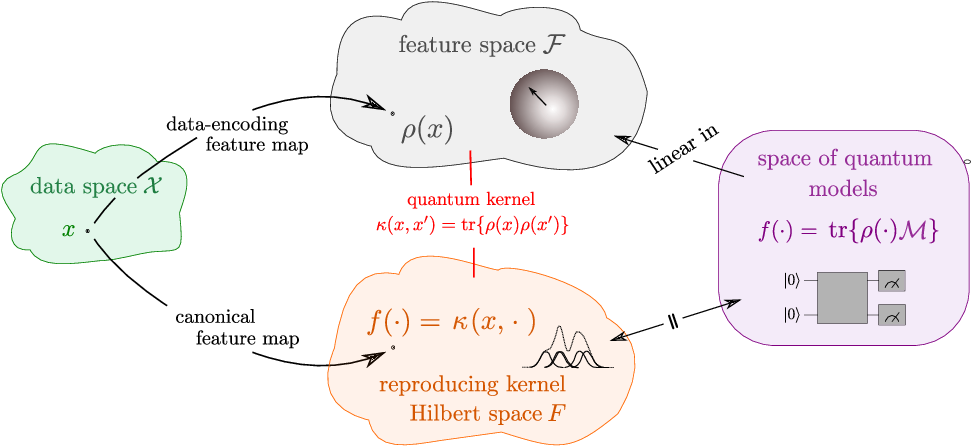
\includegraphics[width=\textwidth]{pics/schuld-overview.png}

\end{frame}


\begin{frame}
  \frametitle{Training with kernels}

  

\end{frame}


\begin{frame}
  \frametitle{Quantum kernel circuits}

  How do we compute quantum kernels on hardware?

\end{frame}

% \section{Conclusion}
% \begin{frame}[fragile]{animation}
%   \vfill
%   Some commands take optional arguments in the form of \verb|<x-y>|,
%   where \verb|x| is the first `sub-frame' on which the context is shown,
%   and \verb|y| is the last. \verb|x| or \verb|y| can be replaced by \verb|+|,
%   referring to `the next sub-frame'. 
%   \vfill
%   \begin{columns}[onlytextwidth]
%   \begin{column}{.5\textwidth}
%     \begin{enumerate}
%       \item<+-> uncovered\ldots
%       \item<+-> one\ldots
%       \item<+-> by\ldots
%       \item<+-> one.
%     \end{enumerate}
%     \end{column}
%   \begin{column}{.5\textwidth}
%       Using only:\only<1>{1}\only<2>{2}\only<3>{3}

%       Using onslide:\onslide<1>{1}\onslide<2>{2}\onslide<3>{3}

%       Using pause:\pause1\pause2\pause3
%   \end{column}
%   \end{columns}
%   \vfill
%   For more advanced animations, see \S 14 of the manual:\\
%   \url{https://www.ctan.org/pkg/beamer}
%   % \url{https://www.ctan.org/pkg/animate}\\
%   % \url{https://www.ctan.org/pkg/media9}
%   \vfill
%   % \transduration{2} automatic progression of slides
%   \transpush<1>
% \end{frame}


\begin{frame}[allowframebreaks,t]{\bibname}
	% the 'I' is caused by 'allowframebreaks'
	\AtNextBibliography{\footnotesize}% or in the preamble \AtBeginBibliography{\small}
	\printbibliography
\end{frame}


\end{document}

